%! Author = WelJo
%! Date = 8/18/2026

\newpage


\section{Methodology: Time-Dependent Functional RoA}
\label{sec:methodology}

% - System Model and Assumptions
%   - System Model: Street network, utility network, critical POIs, discrete time steps, dependencies, flood hazard scenario
%   - Assumptions: Binary power and water availability, road availability via RoA ratio, flooded assets fail, backup lifetime, repair delay
% - Physical Accessibility
% - Functional Utility Supply and Lifetimes
% - Functional POI Score
% - City-Wide Index
% - Topological Coupling
% - Scenario Progression and Simulation Run

To quantify the impact of cascading infrastructure failures on urban resilience, we extend the static RoA index into a dynamic framework.
This framework incorporates temporal flood progression, road-network coupling, utilities like power and water, and facility resilience managed via a finite state machine (FSM).

\subsection{Mathematical Framework of RoA(t)}
\label{subsec:mathematical-framework-of-roa-t}

\subsubsection{Time Deterministic RoA:}
While preserving the standard RoA structure (Equation~\ref{eq:old_roa}), downstream accessibility is dynamically modified by facility functionality, directly governing destination reachability.
We operationalize this as a time-dependent index, $\text{RoA}(\mathcal{C}, t)$, evaluated hourly over the simulation horizon $T$.
Consequently, system states are parameterized continuously over time rather than denoted by static prime notation ($c$ vs. $c'$), where $t_0$ is the baseline and $t$ is any step in the simulation.
The new RoA formula looks as follows:

\begin{equation}
    \text{RoA}(\mathcal{C}, t) = \sum_{j=1}^{m} \left( a_{\mathcal{C},j} \cdot \frac{c(s_{j},d_{j}, t_0)}{c(s_j, d_j, t)} \right)\label{eq:new_roa}
\end{equation}

\noindent
\begin{tabularx}{\textwidth}{@{}l X@{}}
    $\text{RoA}(\mathcal{C}, t)$ & Functional area-wide accessibility index at time $t$ in the simulation. \\
    $\mathcal{C}$ / $m$ & Set ($\mathcal{C}$) and count ($m$) of origin-destination POI connections. \\
    $a_{\mathcal{C},j}$ & Weighting factor of routs j for POI $\mathcal{C}$ subject to $\sum_{j=1}^{m} a_{\mathcal{C},j} = 1$. \\
    $c(s_j, d_j, t_0)$ & Travel cost from origin $s_j$ to destination $d_j$ at initial time $t_0$. \\
    $c(s_j, d_j, t)$ & Travel cost from origin $s_j$ to destination $d_j$ at simulation time $t$.
\end{tabularx}

\subsubsection{Time-Integrated RoA over $T$}
Because $\text{RoA}(\mathcal{C}, t)$ is evaluated continuously over the course of the simulation rather than as a static snapshot, total resilience over the crisis period is captured by the time-integrated RoA ($\text{RoA}_{\text{Int}}$):

\begin{equation}
    \text{RoA}_{\text{Int}}(\mathcal{C}) = \frac{1}{t_N - t_0} \int_{t_0}^{t_N} \text{RoA}(\mathcal{C}, t) \, dt\label{eq:int_roa}
\end{equation}

\noindent
\begin{tabularx}{\textwidth}{@{}l X@{}}
    $\text{RoA}_{\text{Int}}(\mathcal{C})$ & Cumulative time-integrated resilience index over the disaster horizon. \\
    $\mathcal{C}$ & Set of evaluated origin-destination POI connections. \\
    $[t_0, t_N]$ & Analysis period from the start ($t_0$) to the end ($t_N$) of the simulation. \\
    $\frac{1}{t_{\text{end}} - t_{\text{start}}}$ & Normalizing the area under the resilience curve to $[0, 1]$. \\
    $\text{RoA}(\mathcal{C}, t)$ & Time-dependent accessibility index of connections $\mathcal{C}$ at time $t$. \\
    $dt$ & Differential element for integration over time $t$.
\end{tabularx}

\subsection{POI Health: Finite State Machine and State Transitions}
\label{subsec:poi-health-finite-state-machine}

While physical road availability is a necessary condition for accessibility, it is insufficient to guarantee operational functionality.
Facilities such as hospitals and fire stations depend heavily on external utilities (power and water).
When utility grid connections fail, internal backup systems allow temporary operation.
These states and transitions need to be governed by a Finite State Machine (FSM), which bridges also the gap between Kaub et al.\ and Lickert et al.

\subsubsection{FSM States:}
To capture this dynamic functionality, we model each POI $i$ using a four-state FSM where at any time step $t$, the state of a facility is defined as $\sigma_i(t)$, which determines an operational binary indicator $f_i(t) \in \{0, 1\}$ indicating whether a facility can actively accept traffic and deliver service:

\noindent
\begin{minipage}{0.40\textwidth}
    \begin{equation}
        \sigma_i(t) \in \left\{ \begin{aligned}
                                    &\text{Oper}, \text{Depl.}, \\
                                    &\text{Dead}, \text{Rebo.}
        \end{aligned} \right\}\label{eq:states}
    \end{equation}
\end{minipage}%
\begin{minipage}{0.60\textwidth}
    \begin{equation}
        f_i(t) = \begin{cases}
                     1 & \text{if } \sigma_i(t) \in \{\text{Oper.}, \text{Depl.}\} \\
                     0 & \text{if } \sigma_i(t) \in \{\text{Dead}, \text{Rebo.}\}
        \end{cases}\label{eq:binary_indicator}
    \end{equation}
\end{minipage}

\vspace{7mm}

\noindent
\begin{tabularx}{\textwidth}{@{}l X@{}}
    Operational & All external utility connections are active and reserve buffers recharge.
    The facility is fully functional ($f_i(t) = 1$). \\
    Depleting & At least one utility connection has failed while internal reserves bridge the outage.
    The facility remains functional ($f_i(t) = 1$). \\
    Dead & At least one reserve buffer is fully exhausted or the facility site is directly flooded.
    The facility is non-functional ($f_i(t) = 0$). \\
    Rebooting & All utility supply are restored or buffer reserves are above thresholds.
    The facility is non-functional ($f_i(t) = 0$).
\end{tabularx}

\subsubsection{FSM State Transitions and Hysteresis:}
FSM state transitions are governed by resource availability, continuous flood exposure, and hysteresis rules, as summarized in Table~\ref{tab:fsm-state-transitions}.
The parameter $\theta = 0.15$ enforces hysteresis by defining the minimum relative buffer capacity required for a facility to initiate rebooting without full grid restoration, preventing rapid failure-recovery cycling (chattering).
Within each state, transition guards are evaluated sequentially with early-exit semantics: the first condition that evaluates to true triggers the state update, bypassing subsequent guards.


\begin{table}[htbp]
    \centering
    \caption{State transitions and guard conditions governing facility FSM updates (evaluated sequentially with early exit).}
    \label{tab:fsm-state-transitions}
    \renewcommand{\arraystretch}{1.30} % Expands vertical row spacing
    \begin{tabularx}{\textwidth}{l l X}
        \hline
        \textbf{Current State} & \textbf{Next State} & \textbf{Transition Guard Condition} \\
        \hline
        Operational & Dead        & $\mathbf{p}_i \in \text{FloodPolygon}(t)$ \\
        & Depleting   & $\exists r \in \{\text{power}, \text{water}\} : u_{i,r}(t) = 0$ \\
        \hline
        Depleting   & Dead        & $\mathbf{p}_i \in \text{FloodPolygon}(t)$ \\
        & Dead        & $\exists r \in \{\text{power}, \text{water}\} : u_{i,r}(t) = 0 \land b_{i,r}(t) = 0$ \\
        & Operational & $\forall r \in \{\text{power}, \text{water}\} : u_{i,r}(t) = 1$ \\
        \hline
        Dead        & Rebooting   & $\mathbf{p}_i \notin \text{FloodPolygon}(t) \land (\forall r \in \{\text{power}, \text{water}\} : u_{i,r}(t) = 1 \lor b_{i,r}(t) > \theta \cdot B_r)$ \\
        \hline
        Rebooting   & Dead        & $\mathbf{p}_i \in \text{FloodPolygon}(t)$ \\
        & Dead        & $\exists r \in \{\text{power}, \text{water}\} : u_{i,r}(t) = 0 \land b_{i,r}(t) \le \theta \cdot B_r$ \\
        & Operational & $t_{\text{reboot}} \ge T_{\text{repair}} \land (\forall r \in \{\text{power}, \text{water}\} : u_{i,r}(t) = 1)$ \\
        & Depleting   & $t_{\text{reboot}} \ge T_{\text{repair}}$ \\
        \hline
    \end{tabularx}
\end{table}

\subsubsection{FSM Buffer Dynamics:}
Each POI maintains independent reserve buffers $b_{i,r}(t)$ for each resource $r \in \{\text{power}, \text{water}\}$ with maximum capacity $B_r$.
During grid outages ($u_{i,r}(t) = 0$), reserves deplete at the rate $\lambda_r$.
When grid connectivity is restored ($u_{i,r}(t) = 1$), reserves recharge at the rate $\mu_r$:

\begin{equation}
    b_{i,r}(t + 1) = \begin{cases}
                         \max\left(0, \, b_{i,r}(t) - \lambda_r\right) & \text{if } u_{i,r}(t) = 0 \land f_i(t) = 1 \\
                         \min\left(B_r, \, b_{i,r}(t) + \mu_r\right) & \text{if } u_{i,r}(t) = 1 \land f_i(t) = 1
    \end{cases}\label{eq:loss_and_gain}
\end{equation}

\noindent
\begin{tabularx}{\textwidth}{@{}l X@{}}
$b_{i,r}(t), \, B_r$ & Reserve level and max capacity for resource $r$ and PoI $i$ at time $t$. \\
$\lambda_r, \, \mu_r$ & Depletion and recharge rates per unit time for ressource $r$. \\
$u_{i,r}(t)$ & Binary grid connection status for PoI $i$ and resource $r$ at time $t$. \\
$\max, \min$ & Clamping bounds enforcing physical reserve limits $[0, B_r]$.
\end{tabularx}

\subsubsection{Integrated FSM Workflow:} The overall interaction between utility connectivity, reserve buffer dynamics, direct flood overrides, and reboot hysteresis is synthesized in the finite state machine illustrated in Figure~\ref{fig:fsm_state_machine}.

\begin{figure}[htbp]
    \centering
    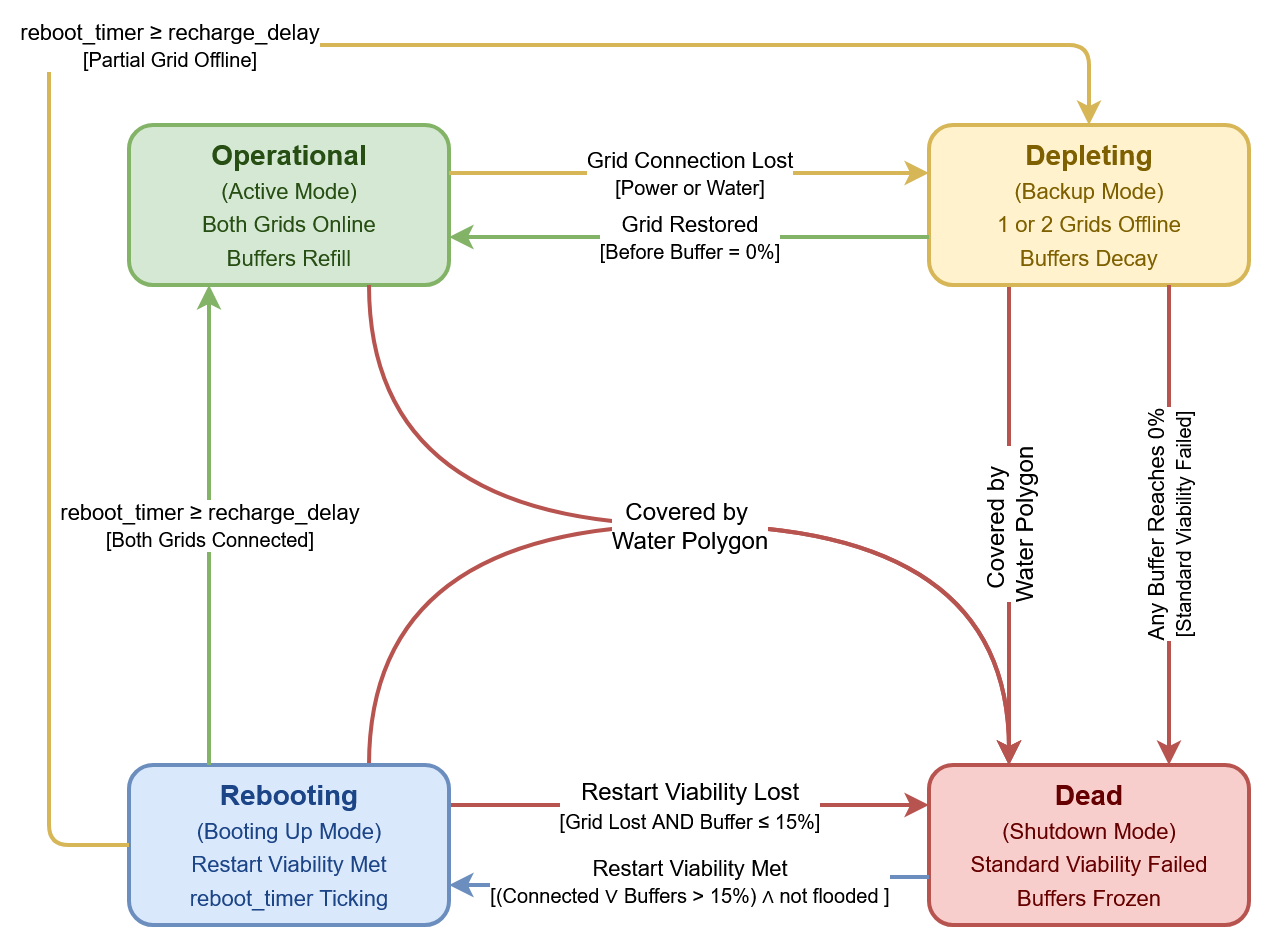
\includegraphics[width=0.9\linewidth]{resources/statemachine}
    \caption{Finite state machine governing POI functional status based on utility connectivity, reserve dynamics, hysteresis thresholds, and environmental flood overrides.}
    \label{fig:fsm_state_machine}
\end{figure}

\subsection{Infrastructure Coupling via NCNN}
\label{subsec:infrastructure-coupling-via-ncnn}


Critical utility networks (power and water) physically follow street corridors underground, despite the individual supply assets and points of interest (POIs) often being located off the road network itself, as highlighted by Okabe et al.\ \cite{okabe2012}
To capture topological barriers without assuming unconstrained Euclidean connectivity, utility dependencies are established using Network-Constrained Nearest-Neighbor (NCNN) mapping over an edge-weighted undirected street graph $G = (V, E)$.
This framework accurately models underlying conduit pathways, enables spatial visualization within the simulation engine, and bridges continuous geographic space with discrete graph topology by projecting off-network entities onto their nearest street network components.
Each POI $i$ is mapped to its topologically closest supply asset $s^*(i, r)$ for resource type $r \in \{\text{power}, \text{water}\}$ via a multi-source shortest-path search:


\begin{equation}
    s^*(i, r) = \arg\min_{s \in \mathcal{I}_r} \text{dist}_G\left(\pi(\mathbf{p}_i), \pi(s)\right)\label{eq:ncnn}
\end{equation}

\noindent
\begin{tabularx}{\textwidth}{@{}l X@{}}
$s^*(i, r)$ & Assigned asset of resource type $r$ topologically closest to facility $i$. \\
$\arg\min_{s \in \mathcal{I}_r}$ & Minimization operator selecting the asset $s$ yielding shortest path. \\
$\mathcal{I}_r$ & Set of active, operational supply assets for resource $r$. \\
$\text{dist}_G(u, v)$ & Shortest network path distance between snapped start vertex $u$ and end vertex $v$ on $G$. \\
$\pi(\mathbf{p}_i), \pi(s)$ & Snapping operators projecting off-network POI ($\mathbf{p}_i$) and asset ($s$) coordinates to graph vertices $u, v \in V$
\end{tabularx}

\vspace{7mm} \noindent
This topological assignment is static and happens only once at the start of the simulation.
A dynamic assignment could be implemented by governing the dynamic grid status $u_{i,r}(t)$ within the facility FSM. :

\begin{equation}
    u_{i,r}(t) = \begin{cases}
                     0 & \text{if } \mathbf{p}_{s^*(i,r)} \in \text{FloodPolygon}(t) \\
                     1 & \text{otherwise}
    \end{cases}\label{eq:u_i_r}
\end{equation}

\noindent
If the assigned supply asset $s^*(i, r)$ is inundated, the utility connection is severed ($u_{i,r}(t) = 0$), initiating buffer depletion ($b_{i,r}$) in the POI's state machine.
